% Presenting LinkML-LiMi
% © 2026 Damien Goutte-Gattat
%
% This work is released under the Creative Commons
% Attribution-ShareAlike 4.0 International License. To view a copy of
% this license, visit https://creativecommons.org/licenses/by-sa/4.0/.
\usepackage{fontspec}
\usepackage{polyglossia}
\usepackage{tikz}
\usepackage{fancyvrb}

\setmainlanguage{english}
\usetheme{Boadilla}
\definecolor{gerbigreen}{RGB}{0,152,57}
\definecolor{gerbidarkgreen}{RGB}{0,146,55}
\definecolor{gerbilightgreen}{RGB}{212,235,220}
\usecolortheme[named=gerbidarkgreen]{structure}
\setbeamertemplate{navigation symbols}{}
\setbeamercovered{transparent}

\AtBeginSection{
  \begin{frame}{Outline}{}
    \tableofcontents[currentsection]
  \end{frame}
}
\graphicspath{{imgs/}{svgs/}}

\title[LiMi in LinkML]{LinkML for the QUAREP-LiMi model}
\author{Damien Goutte-Gattat}
\institute[German BioImaging e.V.]{
\includegraphics[width=4cm]{gerbi-logo}}
\date[QUAREP-LiMi WG, September 2026]{QUAREP-LiMi Working Group, September 2026}

\hypersetup{pdfpagemode=UseNone,
  pdftitle={LiMi in LinkML},
  pdfauthor={Damien Goutte-Gattat}}

\begin{document}

% Frontmatter

\mode<beamer>{
\begin{frame}
  \titlepage
\end{frame}
}


% Contents

\section{On models and schemas}

\begin{frame}
  \frametitle{Data models}

  A data model may describe
  \begin{itemize}
    \item How we \textcolor<2>{red}{think about the data}
    \item How we \textcolor<3>{red}{represent the data in files} (or in a database or similar)
    \item How we represent the data \textcolor<4>{red}{when transmitting them over a network}
    \item How we manipulate the data \textcolor<5>{red}{in a computer program}
  \end{itemize}

  \only<1,6|handout:1>{\hspace{1em}}
  \only<2|handout:0>{(The \textcolor<2>{red}{mental model})}
  \only<3|handout:0>{(The \textcolor<3>{red}{storage model})}
  \only<4|handout:0>{(The \textcolor<4>{red}{exchange model})}
  \only<5|handout:0>{(The \textcolor<5>{red}{in-memory model})}

  \bigskip
  Those different descriptions may not necessarily be aligned
  \begin{itemize}
    \item Whether by choice or by circumstances
  \end{itemize}
\end{frame}

\begin{frame}
  \frametitle{The mental model}

  \begin{itemize}
    \item Ideally comes first
      \begin{itemize}
        \item And influences all other models (storage, exchange, memory)
      \end{itemize}
    \item But not always
      \begin{itemize}
        \item Sometimes the mental model is derived from an existing storage
              model rather than the other way around
      \end{itemize}
  \end{itemize}
\end{frame}

\begin{frame}
  \frametitle{The storage/exchange model(s)}

  \begin{itemize}
    \item May not necessarily be different
    \item Those are the models that are important for \emph{interoperability}
      \begin{itemize}
        \item All software programs that need to manipulate the data files
              and/or send/exchange data through the network must understand the
              same storage/exchange model
      \end{itemize}
    \item This is what the specification for a file format or a network
          protocol must describe
  \end{itemize}

  \bigskip
  \begin{overlayarea}{\textwidth}{3cm}
    \only<2,3,4,5,6|handout:1>{This is \emph{not} the same thing as a serialisation
      format: The \emph{same} storage model can yield different files according
      to different serialisation formats.}
    
    \only<3|handout:1>{
      \begin{block}{Example data model: a point}
\begin{semiverbatim}
struct point \{ int x; int y; \};
\end{semiverbatim}
      \end{block}
    }

    \only<4|handout:0>{
      \begin{block}{Possible serialisation in YAML}
\begin{semiverbatim}
point:

\hspace{2em}x: 123

\hspace{2em}y: 456
\end{semiverbatim}
      \end{block}
    }

    \only<5|handout:0>{
      \begin{block}{Possible serialisation in XML}
\begin{semiverbatim}
<point>

\hspace{2em}<x>123</x>

\hspace{2em}<y>456</y>

</point>
\end{semiverbatim}
      \end{block}
    }

    \only<6|handout:0>{
      \begin{block}{Possible serialisation in X.690 BER}
\begin{semiverbatim}
30 07 02 01 7B 02 02 01 C8
\end{semiverbatim}
      \end{block}
    }

  \end{overlayarea}
\end{frame}

\begin{frame}
  \frametitle{The in-memory model}

  \begin{itemize}
    \item Only concerns one particular software program
      \begin{itemize}
        \item And its plugins, if any (e.g. ImageJ/Fiji)
      \end{itemize}
    \item Different programs can use different in-memory models to manipulate
          the same underlying data
  \end{itemize}
\end{frame}

\begin{frame}
  \frametitle{How to define a data model}

  \begin{block}{As plain human language}
    ``A point has two integers $x$ and $y$, representing its coordinates on the
    X and Y axis respectively.''
  \end{block}

  \begin{block}{As drawings}
    \begin{itemize}
      \item From rough sketches on a napkin to more rigorous schematics
      \item Especially useful for the \emph{mental model} and/or in early design
            phase
      \item Can optionally be quite formal (e.g. \emph{Unified Modeling Language})
    \end{itemize}
  \end{block}

  \begin{block}{As en entirely formal description}
    \begin{itemize}
      \item Using any of several \emph{Schema Definition Languages} (SDLs)
      \item Hereafter, \textcolor<2>{red}{``schema'' = ``a \emph{formal} definition of a data model''}
    \end{itemize}
  \end{block}
\end{frame}

\begin{frame}
  \frametitle{Benefits of a schema}

  \begin{block}{Formality reduces ambiguity}
    \begin{itemize}
      \item Compared to a description in plain English, a schema may be harder
            to understand at first...
      \item But will avoid the ambiguities inherent to human languages
      \item For that reason, a schema may be useful even for a purely mental
            model
    \end{itemize}
  \end{block}

  \begin{block}{Formal = machine-readable}
    Machine-readibility means the schema can enable the partial / full
    automatization of several tasks:
    \begin{itemize}
      \item Generate human-friendly documentation
      \item Generate code (direct translation from mental model to in-memory model)
      \item Validate data (checking that the data fit the model)
    \end{itemize}
    (Not all those features may be available depending on the SDL used)
  \end{block}
\end{frame}

\begin{frame}
  \frametitle{Schema definition languages}

  \begin{itemize}
    \item Abstract Syntax Notation 1 (ASN.1)
    \item Document Type Definition (DTD)
    \item \textcolor<2>{red}{XML Schema}
    \item Schematron
    \item Relax-NG
    \item Concise Data Definition Language (CDDL)
    \item JSON-Schema
    \item JSON Type Definition
    \item \textcolor<2>{red}{LinkML}
    \item ...
  \end{itemize}
\end{frame}

\section{The QUAREP-LiMi model now}

\begin{frame}
  \frametitle{What is the QUAREP-LiMi model?}

  \begin{itemize}
    \item Primarily a \emph{mental model} for now
    \item We want it to become also a storage/exchange model
  \end{itemize}

  \bigskip
  But is it a \emph{model} or a \emph{schema}?
  \begin{itemize}
    \item It is a model...
    \item for which one formal representation (XSD) is available
  \end{itemize}
\end{frame}

\begin{frame}
  \frametitle{How is the LiMi model maintained and edited?}

  \begin{itemize}
    \item The model is maintained as a \textcolor<2>{red}{set of Excel spreadsheets}
      \begin{itemize}
        \item Here: \url{https://github.com/WU-BIMAC/NBOMicroscopyMetadataSpecs}
      \end{itemize}
    \item Other representations must be \textcolor<3>{red}{manually kept in sync}
          with the ``canonical'' spreadsheets
      \begin{itemize}
        \item Formal XML Schema representation
        \item Informative ``Entity-relationship'' diagrams
      \end{itemize}
  \end{itemize}
\end{frame}

\begin{frame}
  \frametitle{The ``canonical'' LiMi model}

  \begin{center}
    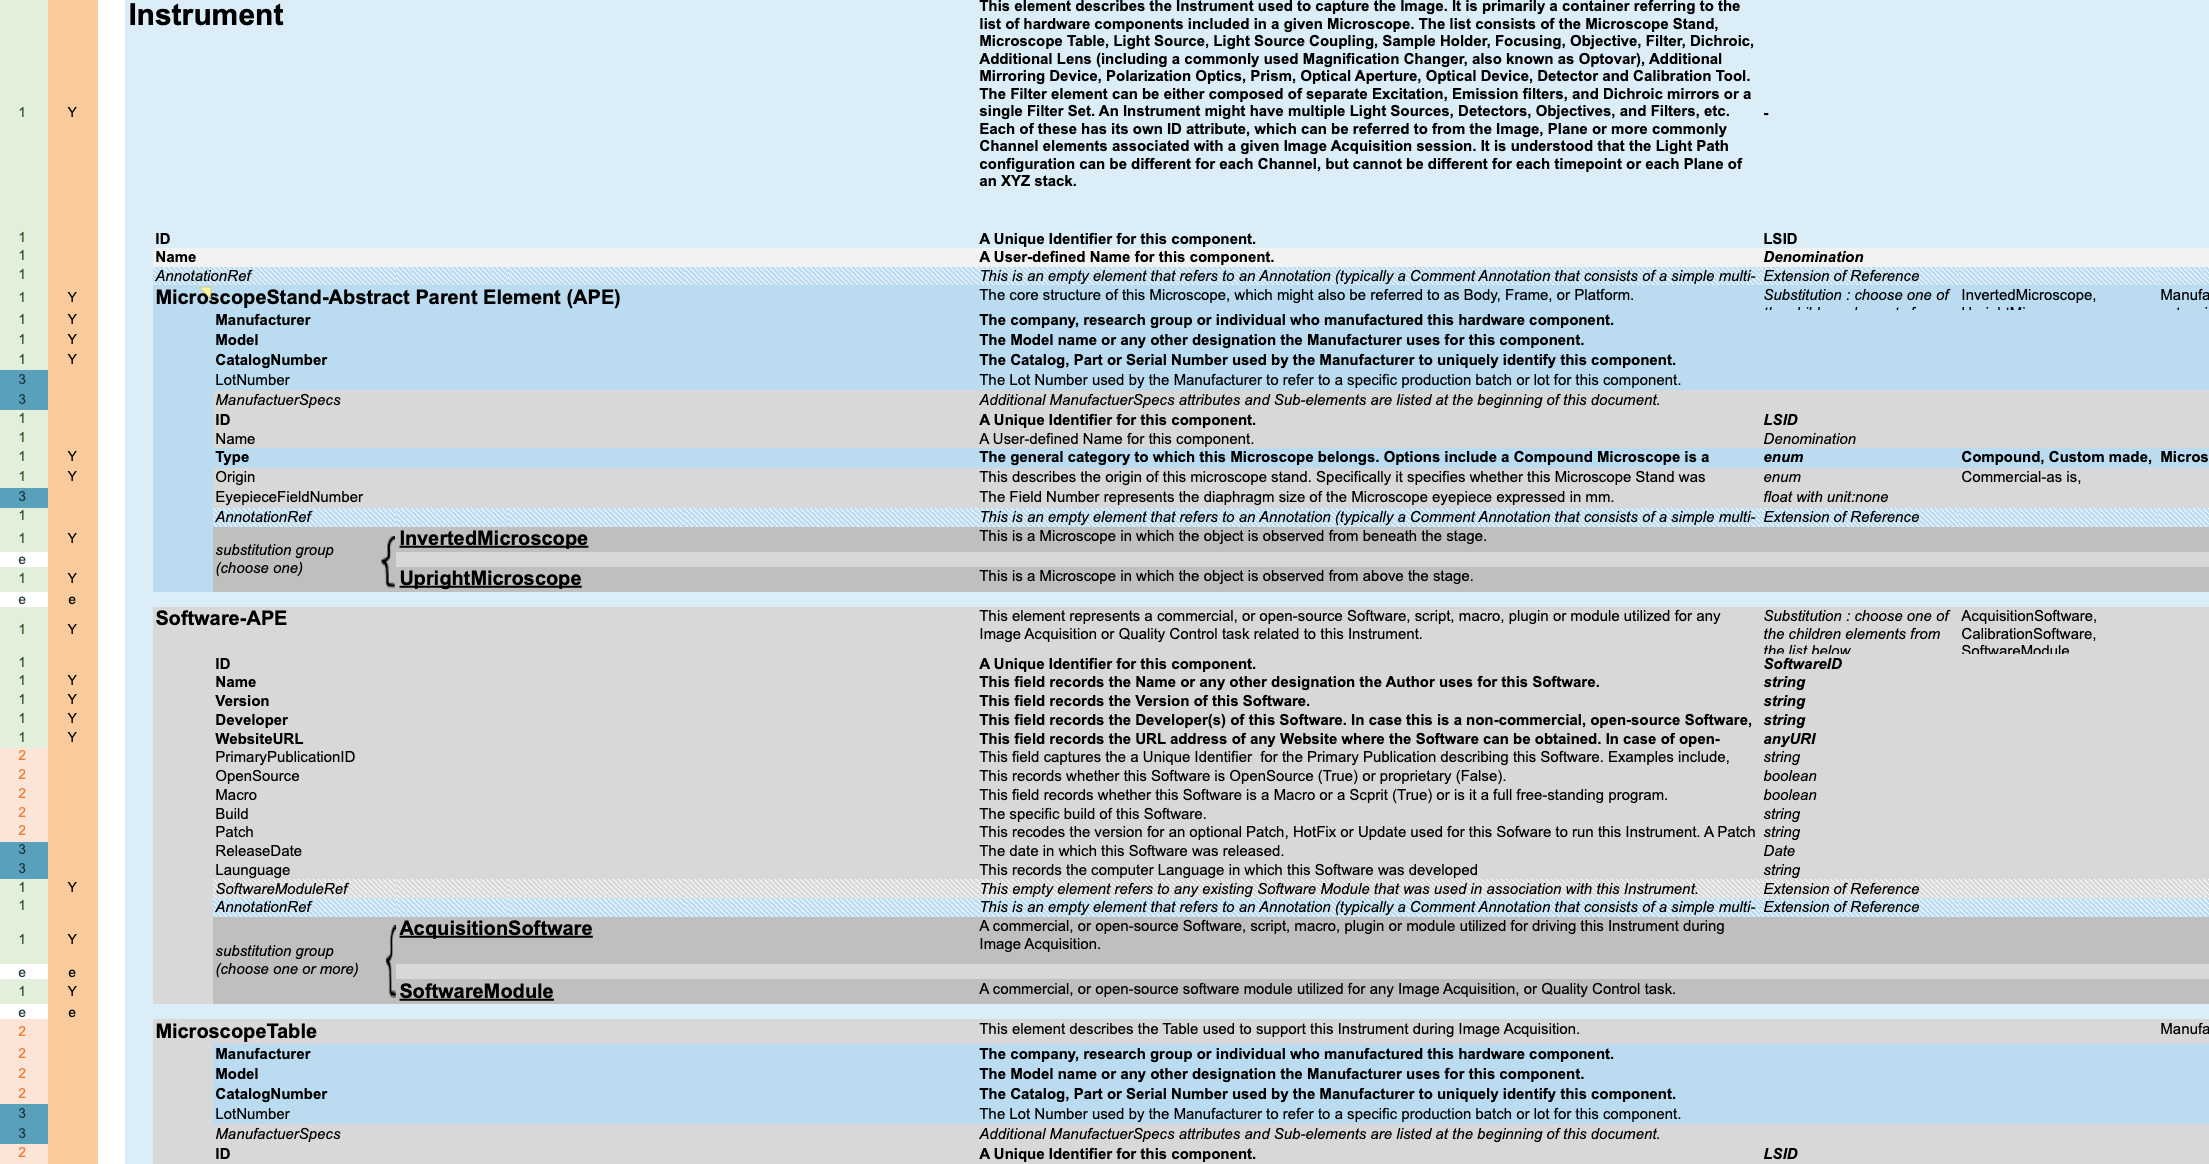
\includegraphics[width=.9\textwidth]{limi-spreadsheet}
  \end{center}
\end{frame}

\begin{frame}
  \frametitle{Excel is not a Schema Definition Language}

  Excel is reasonably easy to use and, with rigorous discipline, can allow a
  certain degree of formalism.

  \bigskip
  However:
  \begin{itemize}
    \item The ease of use becomes relative when dealing with a large model
    \item Even a highly formalized spreadsheet is not enough to make it \emph{machine-readable}
      \begin{itemize}
        \item Other representations \textcolor<2>{red}{cannot be automatically derived}
              from the spreadsheet
        \item \emph{De facto}, there isn't a single source of truth
        \item Keeping the other representations in sync with the spreadsheets is essentially a
              \textcolor<3>{red}{manual process} that is \textcolor<3>{red}{not sustainable}
      \end{itemize}
    \item No consistency checking of any kind
  \end{itemize}
\end{frame}

\begin{frame}
  \frametitle{Why not using XML Schema as the source of truth?}

  \begin{itemize}
    \item XML Schemas are \emph{very} verbose
    \item Specific to XML-formatted data
    \item No easy path towards other representations
  \end{itemize}
\end{frame}

\section{QUAREP-LiMi as a LinkML schema}

\begin{frame}
  \frametitle{About LinkML}

  LinkML aims to be the one true schema definition language.

  \bigskip
  \begin{overlayarea}{\textwidth}{4cm}
    \only<2|handout:1>{
      Mandatory \href{https://xkcd.com/927/}{XKCD:927}
      \begin{center}
        
\includegraphics[width=.6\textwidth]{xkcd927}
      \end{center}
    }

    \only<3|handout:0>{
      \begin{itemize}
        \item LinkML can be translated into several other SDLs
          \begin{itemize}
            \item We can use LinkML without irreversibly tying ourselves to it
          \end{itemize}
        \item Many SDLs are specific to a given type of serialisation formats, e.g.
          \begin{itemize}
            \item DTD: specific to SGML/XML
            \item XML Schema, Relax-NG, Schematron: specific to XML
            \item JSON Schema, JSON Type Definition: specific to JSON
          \end{itemize}
        \item LinkML is independent of any serialisation formats
          \begin{itemize}
            \item YAML/JSON
            \item RDF
            \item CSV
            \item SQL
            \item ...
          \end{itemize}
      \end{itemize}
    }

    \only<4|handout:0>{
      \begin{itemize}
        \item Software support
          \begin{itemize}
            \item Documentation generators
            \item Code generators
            \item Data parsers / writers
            \item Data validators
            \item Other helper tools (e.g. editor support)
          \end{itemize}
      \end{itemize}
    }

    \only<5|handout:0>{
      \begin{itemize}
        \item A reasonably large community has grown around LinkML
          \begin{itemize}
            \item Likely large enough to withstand a withdrawal of the
                  group that created LinkML in the first place, should
                  such a withdrawal ever happen\\
                  (e.g. because of funding cuts)
            \item Independently developed third-party implementations
                  have started to appear
          \end{itemize}
        \item Strong momentum for LinkML in many bio* communities
      \end{itemize}
    }
  \end{overlayarea}

\end{frame}

\begin{frame}
  \frametitle{Anatomy of a LinkML schema}

  A LinkML schema is a YAML file organized in 4 sections:
  \begin{itemize}
    \item A preamble
      \begin{itemize}
        \item Schema-level metadata, e.g. what the schema is about and who
              created it
      \end{itemize}
    \item Class definitions
      \begin{itemize}
        \item Each class represents a type of object in the model
        \item Each class has its own \emph{attributes}
      \end{itemize}
    \item Slot definitions
      \begin{itemize}
        \item Essentially attributes that are used in more than one class,
              and that are therefore declared separately to avoid repeated
              definitions
      \end{itemize}
    \item Enum definitions
      \begin{itemize}
        \item Closed sets of values that can be used elsewhere in the schema
      \end{itemize}
  \end{itemize}
\end{frame}

\begin{frame}
  \frametitle{Class definitions}

\begin{semiverbatim}
classes:

\hspace{1em}LiMiObjective:

\hspace{2em}description: The microscope's Objective lens consists of a

\hspace{3em}lens, its mount, and any associated part [...]

\hspace{2em}attributes:

\hspace{3em}magnification:

\hspace{4em}description: The magnification of the objective as

\hspace{5em}specified by the manufacturer - i.e., 60 represents

\hspace{5em}a 60X lens.

\hspace{4em}range: float

\hspace{3em}correction:

\hspace{4em}description: The type of optical correction associated

\hspace{5em}with this Objective.

\hspace{4em}range: LiMiObjectiveCorrectionType
\end{semiverbatim}
\end{frame}

\begin{frame}
  \frametitle{Enum definitions}

\begin{semiverbatim}
enums:

\hspace{1em}LiMiObjectiveCorrectionType:

\hspace{2em}description: The type of optical correction associated

\hspace{3em}associated with an objective.

\hspace{2em}permissible\_values:

\hspace{3em}Achro:

\hspace{3em}Achromat:

\hspace{3em}Achroplan:

\hspace{3em}Apo:

\hspace{3em}Apochromat:

\hspace{3em}Plan:

\hspace{3em}PlanApo:

\hspace{3em}PlanApochromat:

\hspace{3em}...
\end{semiverbatim}
\end{frame}

\begin{frame}
  \frametitle{``Dynamic enumerations''}

  Defining an enumeration using ontology terms.

\begin{semiverbatim}
enums:

\hspace{1em}Organism:

\hspace{2em}description: The organism a sample comes from.

\hspace{2em}reachable\_from:

\hspace{3em}source\_ontology: obo:NCBITaxon

\hspace{3em}source\_nodes:

\hspace{4em}- NCBITaxon:131567 \# cellular organism

\medskip
\hspace{1em}ImagingMethod:

\hspace{2em}description: The method used to acquire an image.

\hspace{2em}reachable\_from:

\hspace{3em}source\_ontology: obo:FBbi

\hspace{3em}source\_nodes:

\hspace{4em}- FBbi:00000222 \# imaging method
\end{semiverbatim}
\end{frame}

\begin{frame}
  \frametitle{Inline comments and notes}

  \begin{itemize}
    \item Comments: intended for the users of the schema
    \item Notes: intended for the editors of the schema
  \end{itemize}

  \bigskip
  \begin{overlayarea}{\textwidth}{3cm}
    \only<1|handout:1>{
\begin{semiverbatim}
classes:

\hspace{1em}LiMiObjective:

\hspace{2em}attributes:

\hspace{3em}lens\_na:

\hspace{4em}description: The numerical aperture of this Objective.

\hspace{4em}range: float

\hspace{4em}comments:

\hspace{5em}- The value is typically expected to be 0.02 - 1.5.
\end{semiverbatim}}

    \only<2|handout:0>{
\begin{semiverbatim}
classes:

\hspace{1em}LiMiObjective:

\hspace{2em}attributes:

\hspace{3em}correction\_collar:

\hspace{4em}description: Whether this Objective is fitter with

\hspace{5em}a Correction Collar.

\hspace{4em}range: boolean

\hspace{4em}notes:

\hspace{5em}- FIXME This should not be needed? If there is no

\hspace{6em}Correction Collar, then the correction\_collar\_type

\hspace{6em}attribute can simply be left unset.
\end{semiverbatim}}
  \end{overlayarea}
\end{frame}

\begin{frame}
  \frametitle{Custom annotations}

  Any element in a LinkML schema can be annotated with custom,
  structured annotations.

\begin{semiverbatim}
classes:

\hspace{1em}LiMiObjective:

\hspace{2em}description: The microscope's Objective lens consists [...]

\hspace{2em}attributes:

\hspace{3em}magnification:

\hspace{4em}description: The magnification of the objective [...]

\hspace{4em}range: float

\hspace{4em}annotations:

\hspace{5em}recommended\_in\_mm\_section: true
\end{semiverbatim}

  Annotations are an integral part of the schema and are
  accessible by LinkML tools (e.g. documentation generators).

\end{frame}

\begin{frame}
  \frametitle{Sub-schemas}

  Large models can be broken down into several individual LinkML schemas
  (all imported into a ``master'' schema) that are more easily managed 
  than a huge monolithic schema.

  \bigskip
  Current plan for the LiMi model:
  \begin{itemize}
    \item \texttt{limi-core}: ``Core'' LiMi module, broken down into
      \begin{itemize}
        \item \texttt{limi-core-hardware} (``hardware specifications'')
        \item \texttt{limi-core-settings} (``image acquisition settings'')
      \end{itemize}
    \item \texttt{limi-basic}: ``Basic'' LiMi module, similarly broken down into
      \begin{itemize}
        \item \texttt{limi-basic-hardware} (``hardware specifications'')
        \item \texttt{limi-basic-settings} (``image acquisition settings'')
      \end{itemize}
    \item \texttt{limi-advanced}: ``Advanced'' LiMi module
    \item \texttt{limi-confocal}: ``Confocal microscopy'' module
  \end{itemize}
\end{frame}

\begin{frame}
  \frametitle{Summary}

  A LinkML schema
  \begin{itemize}
    \item is reasonably easy to read and edit
    \item is amenable to collaborative editing through GitHub or
          similar forges
    \item can contain all the informations currently found in
          the spreadsheets defining the LiMi model
    \item can be transformed into (almost) anything\\
          (other schemas, code, documentation...)
  \end{itemize}

  \begin{block}{}
    can be the single source of truth defining the LiMi
    model
  \end{block}
\end{frame}

\begin{frame}
  \frametitle{Is LinkML the perfect solution?}

  No.

  \bigskip
  \visible<2,3>{
    \begin{itemize}
      \item Tooling support for languages other than Python is limited
      \item Generated documentation is not necessarily nice to read
      \item Many features are underspecified and therefore best avoided
            for now
    \end{itemize}
  }

  \bigskip
  \visible<3>{
    Those points are being adressed and LinkML can only get better.
  }
\end{frame}


% Backmatter

\mode<beamer>{
\begin{frame}[noframenumbering]
  \frametitle{~}
\end{frame}

\begin{frame}[noframenumbering]
  \frametitle{About}

  \begin{block}{
\includegraphics[scale=.26]{ccbysa}\hspace{.2em}%
    2026 Damien Goutte-Gattat \texttt{<damien@gerbi-gmb.de>}}
    This presentation is released under the Creative Commons
    Attribution-ShareAlike 4.0 International License (CC BY-SA 4.0).
  \end{block}

  \begin{block}{Revision}\ttfamily\scriptsize
    \input{revision.tex}
  \end{block}
  
  \begin{block}{Acknowledgements}
    This work is funded by NSF grant \#2513921
    (``Frameworks-Imaging-PHD'').
  \end{block}
\end{frame}
}

\end{document}
